The combination of CP and search heuristics gives us the \textbf{large neighborhood search}. Large neighborhood search is a hybrid method able to mix together
the benefits coming from the previous strategies. The main idea behind the hybrid approach is described in the following steps:
\begin{enumerate}
    \item Use CP to find an initial solution $s$, exploring a big neighborhood.
    \item Use heuristics to explore different neighborhoods of the initial solution $s$. At the same time, this step is divided into:
    \begin{enumerate}
        \item Keep the assignments already done inside the solution $s$.
        \item Look for the assignments of the remaining decision variables.
    \end{enumerate} \vspace{3.5pt}
    \begin{center}
        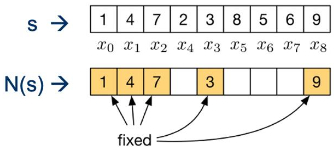
\includegraphics[width = 0.4\textwidth]{img/img27.png}
    \end{center} \vspace{3.5pt}
    As shown in the image above, $s$ is the initial solution, where every decision variable has its own value. Maybe, attempting to improve the initial solution $s$,
    some variables might not have a correspondence anymore. Therefore, we look for new assignments exploring neighborhoods of the initial solution.
\end{enumerate}
We get several advantages coming from the hybrid approach, but the most valuable ones are:
\begin{itemize}
    \renewcommand{\labelitemi}{-}
    \item Efficient neighborhood exploration.
    \item Large neighborhood search is easier to develop than heuristic search.
\end{itemize}